% based on a template made by the university of cologne
% http://www.mi.uni-koeln.de/wp-MIEDV/wp-content/uploads/2016/07/LaTeX-Vorlage.zip - 2023-11-02
\documentclass[12pt,a4paper]{scrartcl}

\addtokomafont{sectioning}{\rmfamily}
\usepackage[ngerman]{babel}% deutsches Sprachpaket wird geladen
\usepackage[T1]{fontenc} % westeuropäische Codierung wird verlangt
\usepackage[utf8]{inputenc}% Umlaute werden erlaubt
\usepackage[usenames]{color} % Erlaubt die Benutzung der namen im Farbpaket und deren Änderung
\usepackage{amsmath} % Erweiterung für den Mathe-Satz
\usepackage{amssymb} % alle Zeichen aus msam und msmb werden dargestellt
\usepackage{graphicx} % Graphiken und Bilder können eingebunden werden
%\usepackage{multirow} % erlaubt in einer Spalte einer Tabelle die Felder in mehreren Zeilen zusammenzufassen
\usepackage{enumerate} % erlaubt Nummerierungen
\usepackage{url} % Dient zur Auszeichnung von URLs; setzt die Adresse in Schreibmaschinenschrift.
\usepackage[center]{caption}  % Bildunterschrift wird zentriert
\usepackage{lmodern}% Für die Schrift
\usepackage[hidelinks]{hyperref} % Links und Verweise werden innerhalb von PDF Dokumenten erzeugt
\usepackage{wrapfig} % Das Paket ermöglicht es von Schrift umflossene Bilder und Tabellen einzufügen.
\usepackage{latexsym} % LaTeX-Symbole werden geladen
\usepackage{tikz} % Erlaubt es mit tikz zu zeichnen
\usepackage{tabularx} % Erlaubt Tabellen
\usepackage{algorithm} % Erlaubt Pseudocode
\usepackage{color} % Farbpaket wird geladen

\numberwithin{equation}{section} % Nummerierungen der Gleichungen, die durch equation erstellt werden, sind gebunden an die section
\newcommand{\HRule}{\rule{\linewidth}{0.7mm}}

% disable commands
\renewcommand{\[}{} % math block start
\renewcommand{\]}{\noindent} % math block end
\newcommand{\tightlist}{} % created in enumerations

\hypersetup{
  pdftitle={B 2.4}
}

% Silbentrennung
\hyphenation{Ent-mag-neti-sier-ungs-ver-hal-ten}
\hyphenation{Ent-mag-neti-sier-ungs-fak-tor}
\hyphenation{Ent-mag-neti-sier-ungs-feld-stär-ke}
\hyphenation{Kom-mu-tie-rungs-kur-ve}
\hyphenation{Grenz-be-reich}
\hyphenation{Mag-ne-ti-sier-ungs-aus-rich-tung}
\hyphenation{er-rei-chen}
\hyphenation{Cu-rie-Tem-pe-ra-tur}

\setcounter{secnumdepth}{6}
\setcounter{tocdepth}{6}

\begin{document}
\begin{titlepage}
	\pagestyle{empty}

	\begin{center}

	\textsc{\LARGE Universität zu Köln }\\ [0.4cm]
	\textsc{Mathematisch-Naturwissenschaftliche Fakultät} \\[1.5cm]

	
\includegraphics[width=0.45\textwidth]{../media/uni}\\[1.5cm]  % Uni-Logo wird geladen

	\textsc{\Large Praktikum~B}\\[2mm]
	\textsc{}\\[10mm]
	\HRule \\[0.4cm]

		{	\Huge \bfseries B 2.4}\\[0.4cm]
			{	\huge \bfseries Magnetisierung eines Ferrits}\\[0.3cm]
	
		\HRule \\[3cm]

		\textsc{\Large Catherine Tran } \\[3pt]
		\textsc{\Large Carlo Kleefisch } \\[3pt]
		\textsc{\Large Oliver Filla } \\[3pt]
		
	\end{center}
\end{titlepage}

\newpage
\tableofcontents

\clearpage
\hypertarget{motivation}{%
\section{Motivation}\label{motivation}}
In diesem Versuch werden Ordnungsphänomene von ferromagnetischen Materialien behandelt. Hierzu werden die Magnetisierungskurven an zwei verschiedenen Aufbauten aufgenommen. Deren zentraler Bestandteil ein Ringkern aus einem Ferrit-Werkstoff ist.

Anhand dieser Kurven lassen sich zahlreiche Eigenschaften dieses Ringkerns untersuchen, wie zum Beispiel die Suszeptibilität, das Temperatur- und das Entmagnetisierungsverhalten.

Mithilfe dieses Versuchs kann ein Einblick in Phänomene des Magnetismus erlangt werden. Dessen Wirkung beschäftigt Menschen schon seit hunderten von Jahren und welcher Grundlage für zahlreiche technische Anwendungen ist.

\clearpage
\hypertarget{theoretische-grundlagen}{%
\section{Theoretische Grundlagen}\label{theoretische-grundlagen}}

\hypertarget{grundlagen-des-magnetismus}{%
\subsection{Grundlagen des Magnetismus}\label{grundlagen-des-magnetismus}}
Das Phänomen des Magnetismus kann nicht klassisch erklärt werden, sondern wird durch die Quantenmechanik beschrieben. Sie befasst sich mit Strömen, was sie qualitativ von der Elektrostatik unterscheidet. Für magnetische Ordnung in ferromagnetischen Materialien ist die
Austauschwechselwirkung verantwortlich, welche auf dem Pauli-Prinzip und der Coulombwechselwirkung beruht.

Die wichtigsten Größen sind die \emph{Flussdichte} \(\vec B\), die \emph{Magnetisierung} \(\vec M\) und die \emph{Feldstärke} \(\vec H\). Diese werden durch die \emph{Feldkonstante}
\(\mu_0=4\pi\cdot 10^{-7}\mathrm{\,\frac{Vs}{Am}}\) bzw. die \emph{Permeabilität} \(\mu\) miteinander in Verbindung gebracht. Die Permeabilität beschreibt die Durchlässigkeit für magnetische Felder. \cite{Jackson}
\begin{eqnarray}
    \vec B &=& \mu_0 \cdot \left(\vec H + \vec M\right) \label{M1}
\end{eqnarray}
Die \emph{Suszeptibilität} \(\chi\) ist eine dimensionslose Größe, welche die Magnetisierbarkeit von Materie beschreibt. Sie beschreibt die Änderung der Magnetisierung \(\vec M\) durch die Änderung der Feldstärke \(\vec H\).
\begin{eqnarray}
    \chi &=& \frac{\mathrm dM}{\mathrm dH} \label{Chi}
\end{eqnarray}
Das magnetische Dipolmoment \(\vec \mu\) tritt auf, wenn elektrische Ladungen sich auf Kreisbahnen bewegen. Es lässt sich über das auf einen magnetischen Dipol wirkende Drehmoment \(\vec \tau\) in einem Magnetfeld \(\vec B\) definieren.

Für eine ebene Leiterschleife ist es folgendermaßen beschrieben. \cite{Jackson}
Die Dichte des magnetischen Momentes wird durch die Magnetisierung beschrieben.
\begin{eqnarray}
    \vec \tau &=& \vec \mu \times \vec B \\
    \vec M &=& \frac{\vec \mu}{V}
\end{eqnarray}
Das Magnetfeld im Inneren einer Spule kann durch den Strom \(I\), die 
Windungszahl \(n\) und die Länge der Spule \(l\) beschrieben werden. Dabei ist \(\vec e_z\) der Einheitsvektor längs der Spule, d.h. senkrecht zur Querschnittsfläche derselben. \cite{Jackson}
\begin{eqnarray}
    \vec H &=& \frac{In}{l} \vec e_z \label{H(I)}
\end{eqnarray}
Für eine einzelne Leiterschleife ist das Magnetfeld dagegen durch die eingeschlossene Fläche \(A\) zu beschreiben, sowie durch den Einheitsvektor \(\vec e_A\) senkrecht zu \(A\).
\begin{eqnarray}
    \vec H &=& IA \vec e_A
\end{eqnarray}

\hypertarget{dia--para--und-ferromagnetismus}{%
\subsection{Dia-, Para- und Ferromagnetismus}\label{dia--para--und-ferromagnetismus}}
Ein \emph{diamagnetischer} Festkörper besitzt keine inneren magnetischen Momente. Durch ein äußeres Magnetfeld werden aber magnetische Momente im Festkörper induziert. Diese sind aufgrund der Lenz'schen Regel dem induzierenden Magnetfeld entgegengesetzt, weshalb die magnetische Suszeptibilität von diamagnetischen Festkörpern \(\mu_\mathrm{dia}\)
negativ ist. Perfekter Diamagnetismus ist bei Supraleitern zu finden. Diese weisen eine magnetische Suszeptibilität von \(\chi_\mathrm{supra} = -1\) auf.

In einem \emph{paramagnetischen} Festkörper liegen innere magnetische Dipolmomente vor, welche z.B. durch Spin und Bahndrehimpuls der Elektronen herrühren. Diese wechselwirken allerdings nicht miteinander, wodurch sie nur in einem äußeren Magnetfeld in Richtung des Feldes ausgerichtet werden. Die magnetische Suszeptibilität \(\chi_\mathrm{para}\) eines paramagnetischen Festkörpers ist daher positiv.

Bei \emph{Ferromagnetismus} sorgt die Austauschwechselwirkung dafür, dass viele benachbarte magnetische Momente parallel zueinander ausgerichtet sind. Ob dies energetisch sinnvoll ist, hängt von der Kombination aus Coulombwechselwirkung und Paulirepulsion ab.

Zudem unterscheidet man noch zwischen Ferrimagnetismus und Antiferromagnetismus. Im \emph{ferrimagnetischen} Material sind die Momente abwechselnd antiparallel zueinander orientiert, dennoch heben sich die Beträge nicht wie im \emph{antiferromagnetischen} Material auf.

\hypertarget{domuxe4nen-und-hysteresekurve}{%
\subsection{Domänen und Hysteresekurve}\label{domuxe4nen-und-hysteresekurve}}
Die im obigen Abschnitt beschriebenen Ordnungsphänomene finden im Material nicht homogen statt. Es existiert also viele einzelne Bereiche mit gleichartigen Magnetisierungsausrichtung, die ``\emph{Weiß'sche Bezirke}'' oder auch ``\emph{Domänen}'' genannt werden. Der Grenzbereich zwischen zwei Weißschen Bezirke heißt \emph{Bloch-Wand}.

Legt man ein kleines, äußeres Magnetfeld an fangen magnetische Momente im Grenzbereich, die energetisch günstiger sind, zuerst ihre Orientierung zu ändern. Kleine Domänen verschmelzen dann zu größeren, dieses Prozess nennt man \emph{Wandverschiebung}.

Wird die Feldstärke höher, finden \emph{Barkhausen-Sprünge} statt. Hierbei ändert sich die Orientierung ganzer Weiß'scher Bezirke schlagartig. Dies geschieht, wenn Defekte in Kristallen zunächst nicht von der Verschiebung der Bloch-Wände betroffen sind. Sind sie fast umringt, so schließt sich die Domäne um den Defekt, wodurch die Magnetisierung sprunghaft ansteigt.

Kurz vor der Sättigung finden \emph{Rotationsprozesse} statt, wo dann alle magnetische Momente in Richtung des äußeren Feldes zeigen.

Die Hysteresekurve beschreibt das Verhalten eines Materials im äußeren Magnetfeld und wird in Abbildung \ref{Abb: Hysteresekurve} schematisch dargestellt. Die Neukurve startet im Ursprung und steigt aufgrund der Wandverschiebungen leicht an, dreht man das Feld auf wird die Kurve wegen der Barkhausen-Sprünge steiler. Bei größer werdenden Feldstärken verläuft sie durch die Rotation wieder flacher zu. Dann findet die Sättigung statt, wo die maximale Magnetisierung erreicht ist.

\begin{figure}[ht]
	\centering
	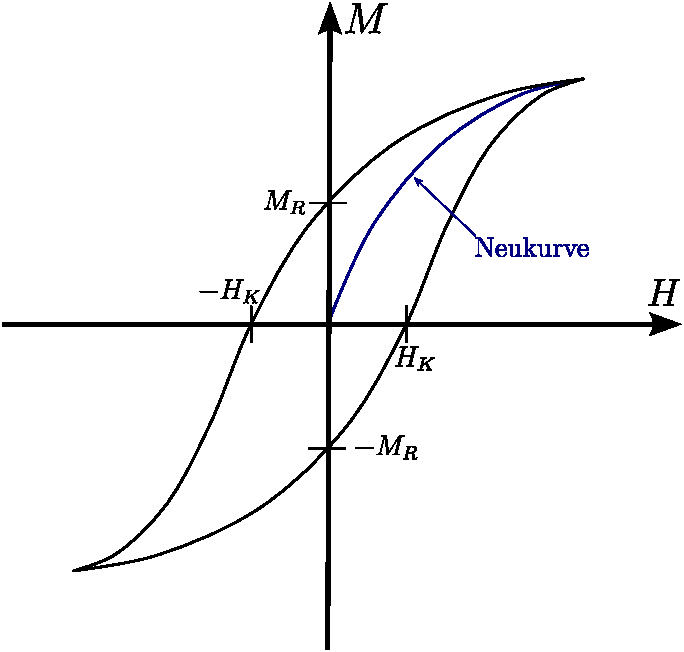
\includegraphics[scale=0.7]{../media/B2.4/Hysteresekurve.pdf}
	\caption{Hysteresekurve}
	\label{Abb: Hysteresekurve}
\end{figure}

Entfernt man das Magnetfeld, sinkt die Magnetisierung nicht automatisch auf null, sondern eine Restmagnetisierung bleibt übrig, die sogenannte \emph{Remanenz}. Soll auch diese verschwinden, muss man ein negatives Feld anlegen und die \emph{Koerzitivfeldstärke} erreichen, der Stoff ist dann vollständig entmagnetisiert. Wird die Feldstärke weiter erhöht, magnetisiert der Stoff in die entgegengesetzte Richtung, bis die Sättigung wieder auftritt.

Die \emph{Kommutierungskurve} ist eine Annäherung der Neukurve. Aus der Kommutierungskurve lässt sich die Suszeptibilität ermitteln.

Die Fläche, die die Hysteresekurve umschließt, entspricht dem Energiegehalt, der beim Umlauf um die Hystereseschleife verloren geht, messbar als Wärme.

Anhand der Hysterese kann man erkennen ob eine Probe weichmagnetisch oder hartmagnetisch ist. \emph{Weichmagnetische} Materialien haben eine kleine Koerzitivfeldstärke und eine hohe Sättigungsmagnetisierung, sie sind also leicht zu magnetisieren. Man verwendet diese oft für Transformatoren und Sensoren.

\emph{Hartmagnetische} Materialien dagegen haben eine große Koerzitivfeldstärke und einen niedrigen Sättigungspunkt. Sie sind schwer zu magnetisieren, daher wird daraus oft Dauermagnete gebaut.

\hypertarget{temperaturabhuxe4ngigkeit-phasenuxfcbergang-und-landau-theorie}{%
\subsection{Temperaturabhängigkeit, Phasenübergang und Landau-Theorie}\label{temperaturabhuxe4ngigkeit-phasenuxfcbergang-und-landau-theorie}}
Magnetische Eigenschaften hängen von der Temperatur ab. Steigt diese an, dann nimmt die Permeabilität ab, also die Ordnung der magnetische Momente. Durch Erhöhung der Temperatur fügt man dem System Energie zu und die Austauschwechselwirkung wird dadurch schwächer, bis sie irgendwann komplett überwunden wird. Dieser Punkt heißt Curie-Temperatur, nur unter dieser Temperatur ist ein ferromagnetischer Stoff einsetzbar. Ab der Curie-Temperatur zeigt der Stoff paramagnetische Verhalten.

Ordnungsparameter beschreibt den Zustand eines System beim Phasenübergang. Bei Ferromagneten ist der Parameter die Magnetisierung. Beträgt der Parameter Null, so ist das System völlig ungeordnet.

Zur Beschreibung von Phasenübergänge dient die Landau-Theorie. Bei der Theorie wird die freie Enthalpie als Funktion der geraden Potenzen der Ordnungsparameter durch Taylorreihenentwicklung ausgedrückt. Beim Gleichgewicht stellt sich die Magnetisierung so ein, dass die freie Enthalpie ihr Minimum einstellt. Daraus wird die Magnetisierung als Funktion der Temperatur bestimmt.

Für \(T=T_\mathrm{C}\) und \(T > T_\mathrm{C}\) ist \(M\approx 0\) und für \(T < T_\mathrm{C}\) gilt \(M = M_0 \cdot \sqrt{T_\mathrm{C} - T}\). Daher wird eine verschobene, an der \(y\)-Achse gespiegelte Wurzelfunktion unterhalb der Curie-Temperatur \(T_\mathrm{C}\) erwartet, die ab der Curie-Temperatur näherungsweise verschwindet.

\hypertarget{entmagnetisierung}{%
\subsection{Entmagnetisierung}\label{entmagnetisierung}}

Laufen die Feldlinien eines äußeren magnetischen Feldes durch die Flächen eines Kristalls, so induzieren sie magnetische Dipolmomente im Kristall. Diesen kann man einen magnetischen Nordpol und einen magnetischen Südpol zuweisen.

Nach der Lenz'schen Regel wirkt das auf diese Weise induzierte Magnetfeld dem äußeren Feld entgegen. Dadurch wird das äußere Feld abgeschwächt, daher nennt man das induzierte Feld auch \emph{Entmagnetisierungsfeld}.

\hypertarget{entmagnetisierungsfaktor}{%
\subsubsection{Entmagnetisierungsfaktor}\label{entmagnetisierungsfaktor}}
Um einen Stoff mit der Magnetisierung \(M\) zu entmagnetisieren, muss ein Entmagnetisierungsfeld \(H_\mathrm{ent}\) angelegt werden. Der Entmagnetisierungsfaktor \(N\) ist der Proportionalitätsfaktor, der den Zusammenhang zwischen dem Entmagnetisierungsfeldes \(H_\mathrm{ent}\) und der Magnetisierung \(M\) eines Materials beschreibt.
\begin{eqnarray}
    N &\equiv& \frac{H_\mathrm{ent}}{M} \label{defN}
\end{eqnarray}
Um die Entmagnetisierung zu erreichen, ohne die interne Magnetisierung \(M\) zu verändern, muss das magnetische Feld \(H_E\) aus dem Medium in Luft verdrängt werden. Dazu kann ein Luftspalt im Medium erzeugt werden. Das Magnetfeld \(H_L\) im Luftspalt wird um den Betrag erhöht, um den das Feld \(H_E\) im Medium verringert wird.
\begin{eqnarray}
    N &=& \frac{l_L}{l} \label{N}
\end{eqnarray}
Dies lässt sich mit einem Ringkern besonders gut realisieren.

\hypertarget{herleitung-des-entmagnetisierungsfaktors}{%
\subsubsection{Herleitung des Entmagnetisierungsfaktors}\label{herleitung-des-entmagnetisierungsfaktors}}
Betrachtet werde ein Ringkern mit dem Ringradius \(R\) und dem Ringquerschnitt mit Radius \(r\) und Fläche \(F_E\). Dieser Ringkern bestehe aus zwei Hälften, die durch einen Luftspalt der Länge \(l_L\) und der Querschnittsfläche \(F_L\). Die mittlere Länge des Rings \(l_E\) sei sehr viel größer als \(l_L\). Weiterhin sei \(R\) sehr viel größer als \(2r\), sodass das Magnetfeld im Ringkern als homogen angenommen werden kann. Auch sei \(l_L\) klein, sodass auch das Magnetfeld im Spalt als homogen angenommen werden kann und der Streufluss vernachlässigbar ist.

Die Spule werde von einer zeitlich konstanten Stromdichte durchflossen. Dadurch lässt sich die Maxwell-Gleichung vereinfachen.
\begin{eqnarray}
    \vec \nabla \times \vec H &=& \vec j
\end{eqnarray}
Mithilfe des Satzes von Stokes können die Feldstärken mit Luftspalt und ohne Luftspalt verglichen werden. Dabei sei \(H\) die Feldstärke ohne Luftspalt. 
\begin{eqnarray}
    H &=& H_E\cdot l_E + H_L \cdot l_L \label{EF1}
\end{eqnarray}
Weil Magnetfelder divergenzfrei ist, müssen die homogenen Felder eine Verbindung zwischen Luftspalt und Ringkern herstellen. Die Anschlussbedingungen fordern folgende Gleichheit. Weil der Streufluss vernachlässigbar sein soll, gilt \(F_E = F_L\), wodurch Gleichheit der Feldstärken folgt.
\begin{eqnarray}
    F_E\cdot B_E &=& F_L\cdot B_L \nonumber \\
    F_E = F_L \Rightarrow B_E &=& B_L \label{EF2}
\end{eqnarray}
Luft wird nicht magnetisiert \((M_L=0)\), der Ringkern dagegen schon \((M_E=M)\). Damit kann man die Materialbeziehungen \(\eqref{M1}\) in die obige Gleicheitsrelation \(\eqref{EF2}\) ein erhält man folgende Relation.
\begin{eqnarray}
    B_E &=& \mu_0 \cdot \left(H_E + M\right) \nonumber \\
    B_L &=& \mu_0 \cdot H_L \nonumber \\
    \Rightarrow H_E + M &=& H_L \label{EF3}
\end{eqnarray}
Durch Einsetzen in \(\eqref{EF1}\) kann man die Feldstärken \(H_E\) und \(H_L\) durch \(H\) und \(M\) darstellen. 
\begin{eqnarray}
    \Rightarrow H_E &=& H - \frac{l_L}{l_E+l_L} M \\
    \Rightarrow H_L &=& H + \frac{l_E}{l_E+l_L} M
\end{eqnarray}
Man sieht, dass die Feldstärke aus dem Ring in den Spalt verdrängt wird, die gesamte Feldstärke bleibt aber erhalten. Die Feldstärke \(H_E\) im Ring wird verringert, der Ring wird also entmagnetisiert.

Da die Magnetisierung \(M\) des Kerns im Versuch konstant bleibt, kann nur \(H\) geändert werden, um \(H_E\) auf \(0\mathrm{\,T}\) zu reduzieren. Daher muss das Entmagnetisierungsfeld \(H_\mathrm{ent}\) angelegt 
werden, um \(H_E\) zu verringern. Dadurch kann man den Entmagnetisierungsfaktor \(N\) durch seine Definition \(\eqref{defN}\) bestimmen. 
\begin{eqnarray}
    H_\mathrm{ent} &=& \frac{l_L}{l_E+l_L} M \\
    N &=& \frac{l_L}{l_E+l_L} = \frac{l_L}{l}
\end{eqnarray}

\hypertarget{gescherte-hysteresekurve}{%
\subsubsection{gescherte Hysteresekurve}\label{gescherte-hysteresekurve}}
Das äußere Magnetfeld \(H\) wird über die Stromstärke gemessen, die Magnetisierung \(M\) des Ringkerns wird konstant gehalten. Das Magnetfeld \(H\) muss um ein Entmagnetisierungsfeld \(H_\mathrm{ent}\) erhöht werden, um das innere Magnetfeld \(H_E\) des Kerns zu negieren. Die benötigte Stärke von \(H_\mathrm{ent}\) hängt von der Breite des Luftspalts ab, was aus dem Entmagnetisierungsfaktor hervorgeht, siehe Gleichung \(\eqref{N}\).

In einem Ringkern ohne Luftspalt entspricht die Stärke des äußeren Magnetfeldes \(H\) der des inneren Magnetfeldes \(H_E\). Mit einem Luftspalt steigt \(H\) an, somit wird die Hystereseschleife nach außen geschert. Daher lässt sich \(H_\mathrm{ent}\) durch die Scherung der Hystereseschleife bestimmen. 
\begin{eqnarray}
    H_\mathrm{ent} &=& H - H_E \label{Hscher}
\end{eqnarray}

\clearpage
\hypertarget{durchfuxfchrung}{%
\section{Durchführung}\label{durchfuxfchrung}}
Dieser Versuch besteht aus zwei Teilen. Zunächst werden Messungen am beheizbaren Ferritkern durchgeführt, danach Messungen am Ferritkern mit Spalt. Diese lassen sich wiederum in die einzelnen Messungen aufteilen, welche im Folgenden besprochen werden.

\hypertarget{versuchsaufbau}{%
\subsection{Versuchsaufbau}\label{versuchsaufbau}}
Im Zentrum dieses Versuchs befinden sich zwei unterschiedliche Ferritkerne dessen Magnetisierung untersucht wird. Der erste ist ein beheizbarer Kern, welcher erhitzt werden kann, um Temperaturabhängigkeiten messbar zu machen. Der zweite Kern ist in der Hälfte geteilt und es lässt sich ein Spalt variabler Breite einstellen, was es möglich macht, den Entmagnetisierungsfaktor zu bestimmen.

Beide Ringkerne haben einen Querschnitt von \(q=0.9\,\mathrm{cm^2}\) und einen Kernradius von \(R=1.5\,\mathrm{cm}\). Sie sind von jeweils zwei Spulen umwickelt, einer Primärspule und einer Sekundärspule, deren Windungszahlen sich je nach Kern unterscheiden. Beim beheizbaren Kern haben beide Spulen eine Windungszahl von \(17\). Beim Ringkern mit Spalt hat die Sekundärspule ebenfalls eine Windungszahl von \(17\), die Primärspule allerdings eine von \(54\).

\hypertarget{versuchsidee}{%
\subsection{Versuchsidee}\label{versuchsidee}}
In der Grundidee des Versuchs wird an die Primärspule ein Strom angelegt. Der dadurch in der Sekundärspule induzierte Strom \(U_M\) hängt mit der Magnetisierung \(M\) des Kerns zusammen.
\begin{eqnarray}
    U_M &=& -n_s q \mu_0 \frac{\mathrm dM}{\mathrm dt}
\end{eqnarray}
Der Anteil des Magnetfeldes in der Sekundärspule, das vom Feld im Raum zwischen Kern und Spulenwicklung herrührt, wird dabei von einem Lufttransformator herausgefiltert. Für jeweils Primär- und Sekundärspule ist dies eine Spule ohne Kern, welche andersherum gewickelt und in Reihe geschaltet ist. Der Anteil des Magnetfeldes im Raum zwischen Kern und Spulenwicklung werden also zweimal erzeugt, nur einmal mit anderem Vorzeichen. Sie kürzen sich also genau heraus.

\hypertarget{integration-des-messsignals}{%
\subsubsection{Integration des Messsignals}\label{integration-des-messsignals}}
Um nun \(M\) zu bestimmen, wird das einlaufende \(U_M\) mittels eines Integrators zeitlich integriert und es folgt \(M(t)\) bis auf eine Konstante \(M(0)\). 
\begin{eqnarray}
    U_\mathrm{aus}(t)
        &=& -\frac{1}{R C} \int_{0}^{t} U_M(t^{\prime}) \mathrm dt^{\prime} \\
        &=& -\frac{n_s q}{R C} \mu_0 (M(t) - M(0))
\end{eqnarray}
Ein Integrator ist dabei ein technisches Bauteil, bestehend aus einem Widerstand, einer Diode und einem Kondensator, welcher eine einlaufende Spannung, wie der Name schon sagt, zeitlich integriert. 

\hypertarget{transformation-des-messsignals}{%
\subsubsection{Transformation des Messsignals}\label{transformation-des-messsignals}}
Aufgrund der hohen Frequenz der Wechselspannung von \(50\,\mathrm{Hz}\) wird eine Hysteresekurve nun allerdings viel zu schnell durchlaufen, um eine geeignete Messung dieser zu ermöglichen. Dazu wird mit Hilfe zweier phasenempfindlicher Gleichrichter das Messpaar \((H(t), M(t))\) zu \((H(\varphi), M(\varphi))\) transformiert, was eine langsamere Abtastung der Kurve möglich macht.

\hypertarget{bestimmung-von-mvarphi}{\label{bestimmung-von-mvarphi}}
Ein phasenempfindlicher Gleichrichter multipliziert zum einlaufenden Messsignal \(U_E\) eine zweite sogenannte Referenzspannung \(U_R\) mit einer leicht unterschiedlicher Frequenz hinzu und bildet den zeitlichen Mittelwert. Es entsteht ein Signal, das die Hysteresekurve langsam durchfährt, wobei die Geschwindigkeit proportional zur Differenz der Mess- und Referenzfrequenz ist. Dies wird als ``\emph{freilaufender Betrieb}'' bezeichnet.
\begin{eqnarray}
    M(t) &=& M(\varphi(t))
\end{eqnarray}
Werden die beiden Frequenzen gleichgesetzt, lässt sich durch Änderung der Phasenverschiebung der beiden Signale die Hysteresekurve manuell abtasten oder bestimmte Punkte auf der Hysteresekurve ansteuern, was ``\emph{Phase-Locked-Betrieb}'' genannt wird.
\begin{eqnarray}
    M(t) &=& M(\varphi)
\end{eqnarray}
\hypertarget{bestimmung-von-hvarphi}{\label{bestimmung-von-hvarphi}}Um nun die Hysteresekurve auftragen zu können, muss neben \(M(\varphi)\) noch \(H(\varphi)\) bestimmt werden. Dazu wird ein Transformator ohne Eisenkern, auch Luftinduktorium genannt, mit dem Stromkreis des Kerns in Reihe geschaltet. Die induzierte Spannung in der Sekundärseite des Luftinduktoriums ist proportional zu \(\frac{\mathrm dH}{\mathrm dt}\), wodurch mit dem gleichen Prinzip wie bei der Magnetisierung zuvor \(H(\varphi)\) bestimmt wird.

Mittels des Wertepaars \((M(\varphi), H(\varphi))\) is die Hysteresekurve nun abbildbar.

\hypertarget{messung-am-beheizbaren-ferritkern}{%
\subsection{Messung am beheizbaren Ferritkern}\label{messung-am-beheizbaren-ferritkern}}

\hypertarget{magnetisierungskurve}{%
\subsubsection{Magnetisierungskurve}\label{magnetisierungskurve}}
Im ersten Teil des Versuchs werden bei Zimmertemperatur die Magnetisierungskurven für verschiedene eingestellte Primärstromstärken zwischen \(3\,\mathrm A\) und \(0.1\,\mathrm A\) gemessen. Die Messung findet im freilaufenden Betrieb statt, damit \(\varphi(t)\) über eine gewisse Zeit die ganze Kurve abdeckt.

\hypertarget{kommutierungskurve}{%
\subsubsection{Kommutierungskurve}\label{kommutierungskurve}}
Daraufhin wird die Kommutierungskurve angenähert, indem der obere Umkehrpunkt der Hysteresekurve als Funktion des Primärstroms ermittelt wird. Dazu wird in den Phase-Locked-Betrieb gewechselt und \(\varphi\) wird so eingestellt, dass sich der Messpunkt auf dem Umkehrpunkt befindet. Dann wird während aktiver Messung der Primärstrom vom Maximum \(3\,\mathrm A\) langsam auf \(0\,\mathrm A\) reduziert.

Um den unteren Teil der Kommutierungskurve noch genauer aufzunehmen, wird der Bereich von \(0.1\,\mathrm A\) bis \(0\,\mathrm A\) mittels Feinjustierung der Stromstärke erneut aufgenommen.

\hypertarget{temperaturabhuxe4ngigkeit}{%
\subsubsection{Temperaturabhängigkeit}\label{temperaturabhuxe4ngigkeit}}
Die letzte Messung am beheizbaren Ferritkern beschäftigt sich mit der Temperaturabhängigkeit der maximalen Magnetisierung \(M(T)\). Dazu wird erneut \(\varphi\) im Phase-Locked-Betrieb so eingestellt, dass der Messpunkt auf dem oberen Umkehrpunkt der Hysteresekurve liegt. Außerdem wird der Primärstrom auf den maximalen Wert von \(3\,\mathrm A\) gestellt und der Heizstrom angeschlossen.

Bei aktiver Messung von wird der Ferritkern langsam aufgeheizt bis ein Phasenübergang zu erkennen ist, wobei der Heizstrom aufgrund von steigender Wärmeverluste stetig erhöht werden muss.

\hypertarget{messungen-am-ringkern-mit-spalt}{%
\subsection{Messungen am Ringkern mit Spalt}\label{messungen-am-ringkern-mit-spalt}}

\hypertarget{magnetisierungskurve-1}{%
\subsubsection{Magnetisierungskurve}\label{magnetisierungskurve-1}}

Für den Ferritkern mit Spalt wird zunächst auch die Magnetisierungskurve gemessen. Dies geschieht bei einer Stromstärke von \(0.94\,\mathrm A\), um die Kurve der beiden Ferritkerne später möglichst gut vergleichen zu können.

\hypertarget{entmagnetisierungsfaktor-1}{%
\subsubsection{Entmagnetisierungsfaktor}\label{entmagnetisierungsfaktor-1}}
In der letzten Messung des Versuchs werden mehrere Magnetisierungskurven für unterschiedliche Spaltbreiten von \(0\,\mathrm{mm}\) bis \(1\,\mathrm{mm}\) aufgenommen. Dabei wird für jede Spaltbreite den Primärstrom so eingestellt, dass die maximale Magnetisierung für alle Spalte gleich ist. Begonnen wird bei einer Spaltbreite von \(1\,\mathrm{mm}\) und Primärstrom von \(3\,\mathrm A\).

Hierbei ist zu beachten, dass der Ringkern an zwei Stellen unterbrochen wird. Dadurch ist die Länge \(l_L\) des Luftspalts doppelt so groß, da beide Spalte addiert werden.

\clearpage
\hypertarget{auswertung}{%
\section{Auswertung}\label{auswertung}}

\hypertarget{messungen-am-beheizbaren-ringkern}{%
\subsection{Messungen am beheizbaren
Ringkern}\label{messungen-am-beheizbaren-ringkern}}

\hypertarget{kenngruxf6uxdfen}{%
\subsubsection{Kenngrößen}\label{kenngruxf6uxdfen}}
Zunächst müssen die gemessenen Werte in die richtigen Einheiten konvertiert werden. Gemessen wurden Spannungen, diese müssen in die Magnetisierung \(M\) bzw. die magnetische Feldstärke \(H\) umgerechnet werden.

Die Umrechnung in die Feldstärke kann mittels der Relation \(\eqref{H(I)}\) erfolgen. Der Strom \(I\) kann über das Ohm'sche Gesetz \(U=RI\) aus der Spannung \(U\) und dem Widerstand \(R\) ermittelt werden. Da der Widerstand konstant ist, kann er durch das Verhältnis der maximalen Stromstärke \(I_\mathrm{max}\) und der maximalen Spannung \(U_\mathrm{max}\) beschrieben werden. Weiterhin wird die Länge \(l\) der Spule benötigt. Diese entspricht dem Umfang des Ringkerns, also \(l=2\pi R\) für einen Kern mit dem Radius \(R=1.5\mathrm{\,cm}\). Damit kann die Feldstärke \(H\) wie folgt ermittelt werden.
\begin{eqnarray}
    H &=&
        \frac{n_p}{2\pi R} \cdot \frac{I_\mathrm{max}}{U_\mathrm{max}} \cdot U
        \label{H}
\end{eqnarray}
Aus der Versuchsanleitung \cite{Uni} folgt, dass die Magnetisierung \(M\) aus der gemessenen Spannung \(U\) ermittelt werden kann. Hierbei sind \(\nu=\mathrm{50\,Hz}\) die Frequenz des Wechselstroms, \(n_s=17\) die Windungszahl der Sekundärspule und \(q = \mathrm{0.9\,cm^2}\) die
Querschnittsfläche des Kerns.
\begin{eqnarray}
    M &=&
        \frac{U}{47\cdot 4\nu n_s q \mu_0}
        \label{M}
\end{eqnarray}
Die entsprechenden Messergebnisse werden in Abbildung \ref{Abb: heizbar kenngrößen} und Tabelle \ref{Tab: heizbar kenngrößen} dargestellt. Es ergeben sich folgende Kenngrößen, die aus den Daten abgelesen werden können. Als Fehler werden hierbei die Differenzen der beiden Messwerte auf beiden Seiten der Kurve verwendet.

Man sieht, dass die Remanenz und die maximale Magnetisierung mit
steigender Stromstärke \(I_\mathrm{max}\) zunehmen, was den Erwartungen
entspricht. Selbiges gilt für die Koerzitivfeldstärke \(H_\mathrm{K}\),
wenngleich diese im Rahmen der Ungenauigkeit nahezu konstant bleibt.

\begin{figure}[ht]
\centering
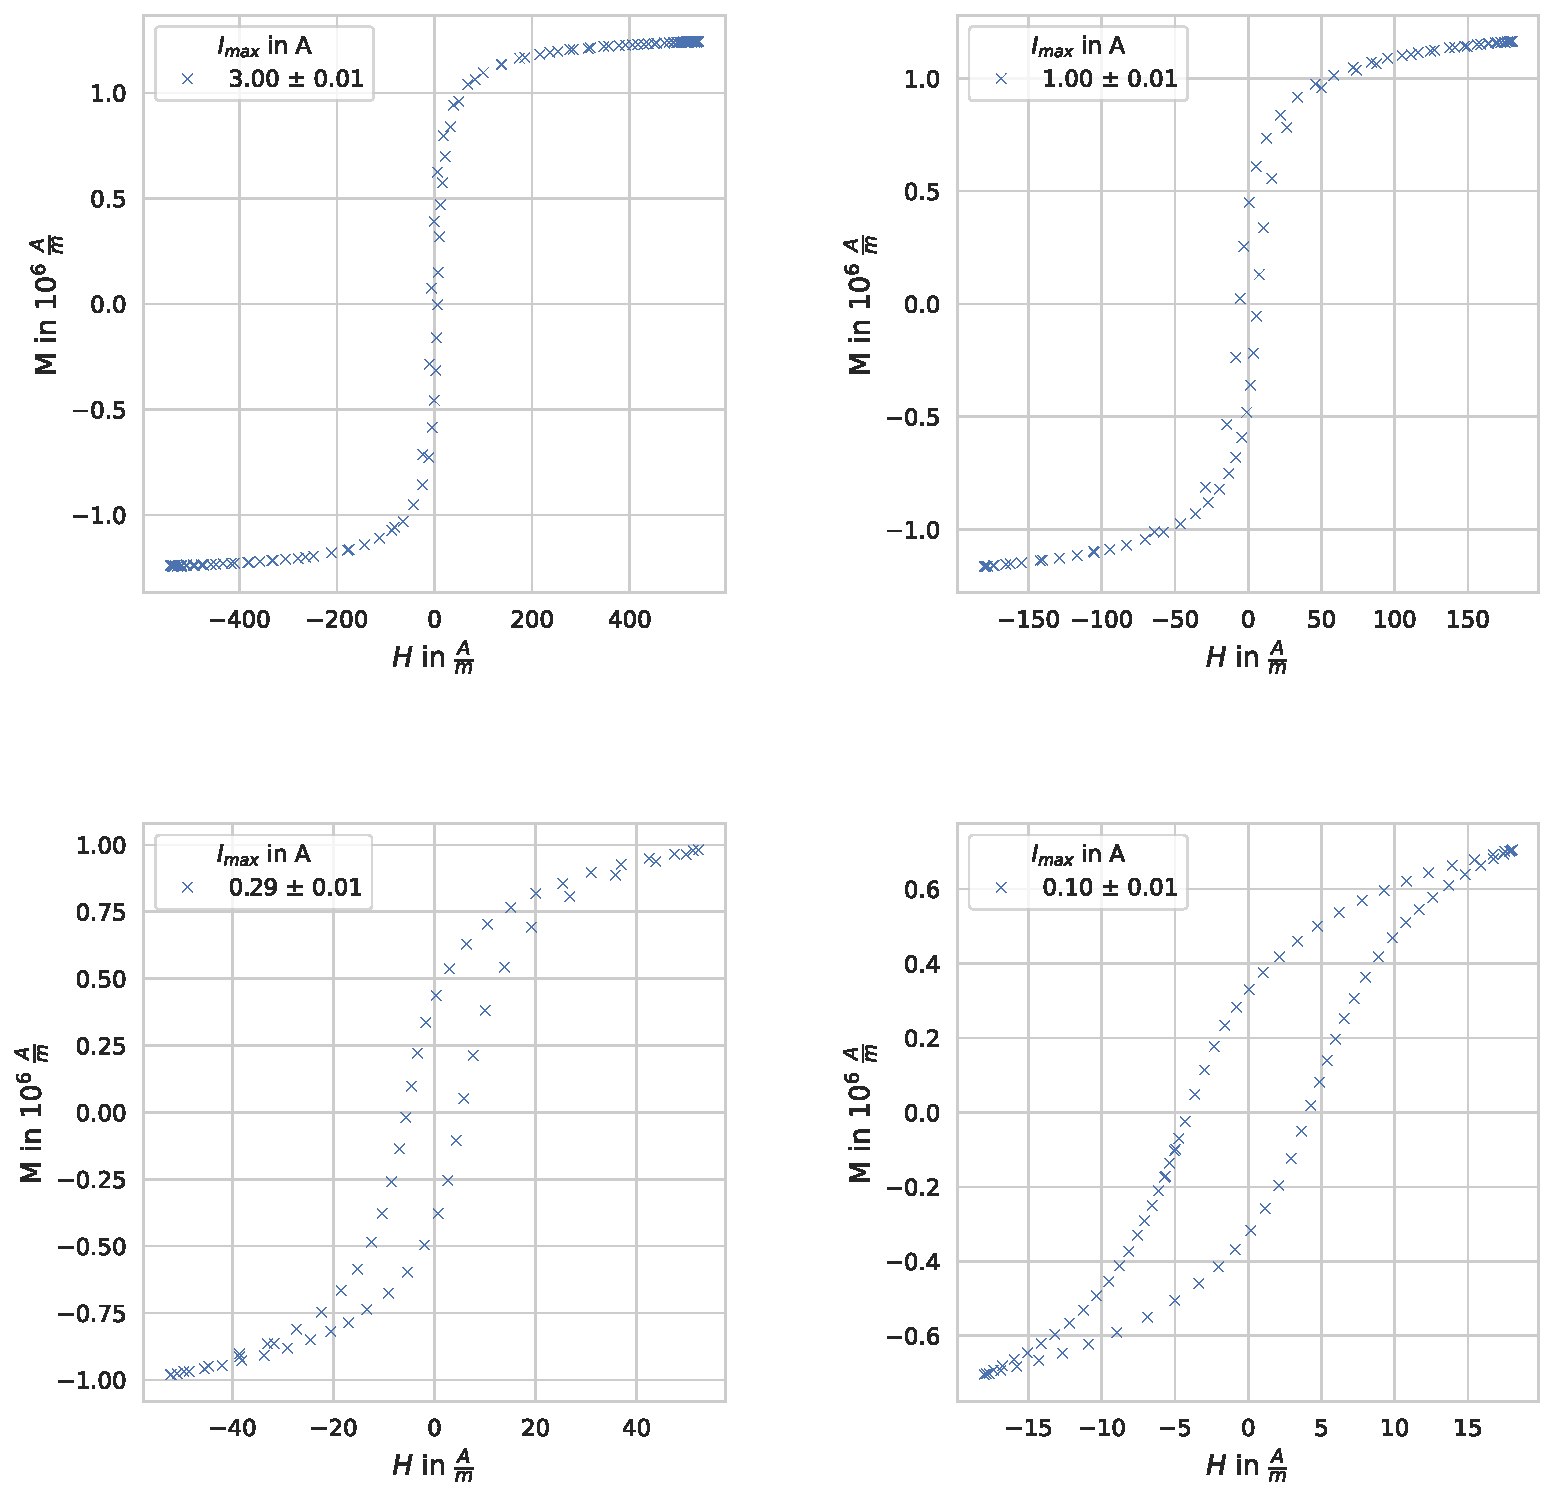
\includegraphics[scale=0.6]{../media/B2.4/3.3.1_single_measures.pdf}
\caption{Einzelne Messungen der Kenngrößen}
\label{Abb: heizbar kenngrößen}
\end{figure}

\begin{table}
	\begin{align*}
		I_\mathrm{max} &\text{ in } A &
		H_\mathrm{K} &\text{ in }
		{\tiny \left[ \frac{A}{m} \right] } &
		M_\mathrm{R} &\text{ in }
		{\tiny \left[10^6  \frac{A}{m} \right] } &
		M_\mathrm{max} &\text{ in }
		{\tiny \left[10^6 \frac{A}{m} \right] }
		\\
		3.00 &\pm 0.01 &
			5.71 &\pm 0.46 &
			0.11 &\pm 0.04 &
			0.31 &\pm 0.08
			\\
		1.00 &\pm 0.01 &
			5.55 &\pm 0.08 &
			0.12 &\pm 0.05 &
			0.29 &\pm 0.09
			\\
		0.29 &\pm 0.01 &
			5.37 &\pm 0.67 &
			0.10 &\pm 0.55 &
			0.25 &\pm 0.11
			\\
		0.10 &\pm 0.01 &
			4.29 &\pm 0.03 &
			0.08 &\pm 0.06 &
			0.18 &\pm 0.12
	\end{align*}
	\caption{Kenngrößen des beheizbaren Ringkerns}
	\label{Tab: heizbar kenngrößen}
\end{table}

\hypertarget{kommutierungskurve-und-suszeptibilituxe4t}{%
\subsubsection{Kommutierungskurve und Suszeptibilität}\label{kommutierungskurve-und-suszeptibilituxe4t}}
Die Kommutierungskurven verlaufen grundsätzlich wie erwartet, siehe Abbildung \ref{Abb: kommut}. Allerdings ist auffällig, dass die Kurve für \(I_\mathrm{max}=100\mathrm{\,mA}\) in eine negative Magnetisierung läuft, was sie von der Kurve für \(I_\mathrm{max}= 3\,\mathrm A\) unterscheidet. Dies deutet auf einen systematischen Fehler bei der erstgenannten Messung hin. Vermutlich ist die Phase während der Messung verrutscht.

Dies wirkt sich auch auf die differentielle Suszeptibilität \(\chi\) aus, siehe Abbildung \ref{Abb: diff kommut}. Bei der Messung mit \(I_\mathrm{max}= 3\,\mathrm A\) ist eine Abhängigkeit von \(\chi \propto H^{-1}\) zu erkennen. Die differentielle Suszeptibilität für die Messung bei \(I_\mathrm{max}=100\mathrm{\,mA}\) hat dagegen sehr viel kleinere Werte, die um einen Faktor von mindestens 20 kleiner sind. Auch dies lässt auf einen systematischen Fehler schließen. Ansonsten ist auch diese Kurve gespiegelt, was mit der negativen Magnetisierung zusammenhängt.

\begin{figure}[ht]
	\centering
	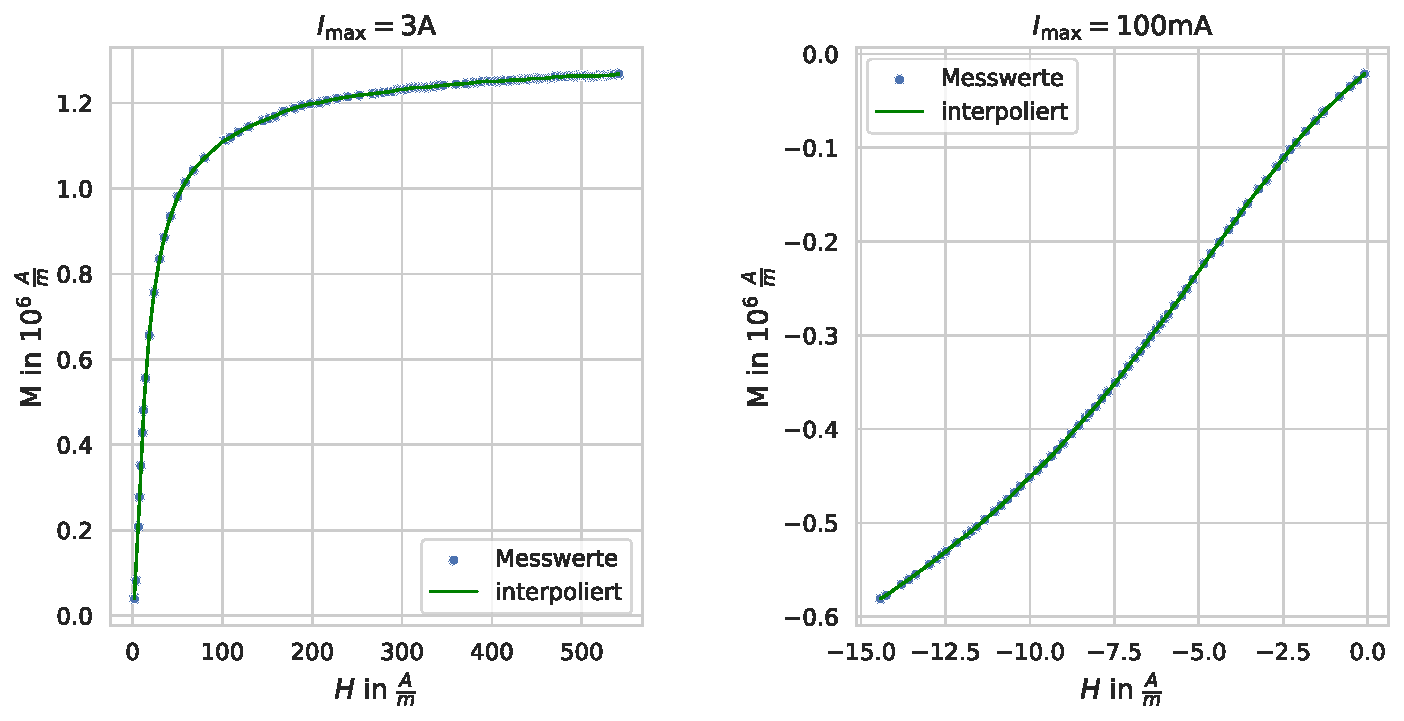
\includegraphics[scale=0.6]{../media/B2.4/3.3.2_Messung.pdf}
	\caption{Kommutierungskurven}
	\label{Abb: kommut}
\end{figure}

\begin{figure}[ht]
	\centering
	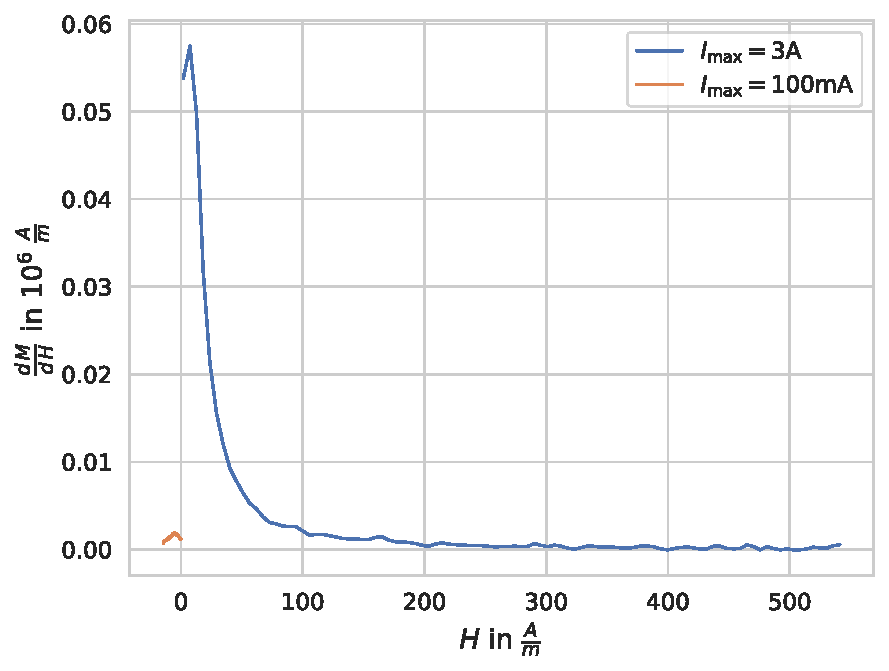
\includegraphics[scale=0.7]{../media/B2.4/3.3.2_Ableitung.pdf}
	\caption{Ableitungen der Kommutierungskurven}
	\label{Abb: diff kommut}
\end{figure}

\hypertarget{temperaturabhuxe4ngigkeit-1}{%
\subsubsection{Temperaturabhängigkeit}\label{temperaturabhuxe4ngigkeit-1}}
Die Magnetisierung \(M(T)\) ist wie erwartet eine abfallende Kurve. Bei der Curie-Temperatur \(T_C\) findet ein Phasenübergang statt, bei dem das Material praktisch paramagnetisch wird. Daher kann man \(T_C\) am unteren Knick ablesen, siehe Abbildung \ref{Abb: Temperatur}.
\begin{eqnarray*}
    T_C &=& (76.5 \pm 0.5) \ ^\circ\mathrm C
\end{eqnarray*}

\begin{figure}[ht]
\centering
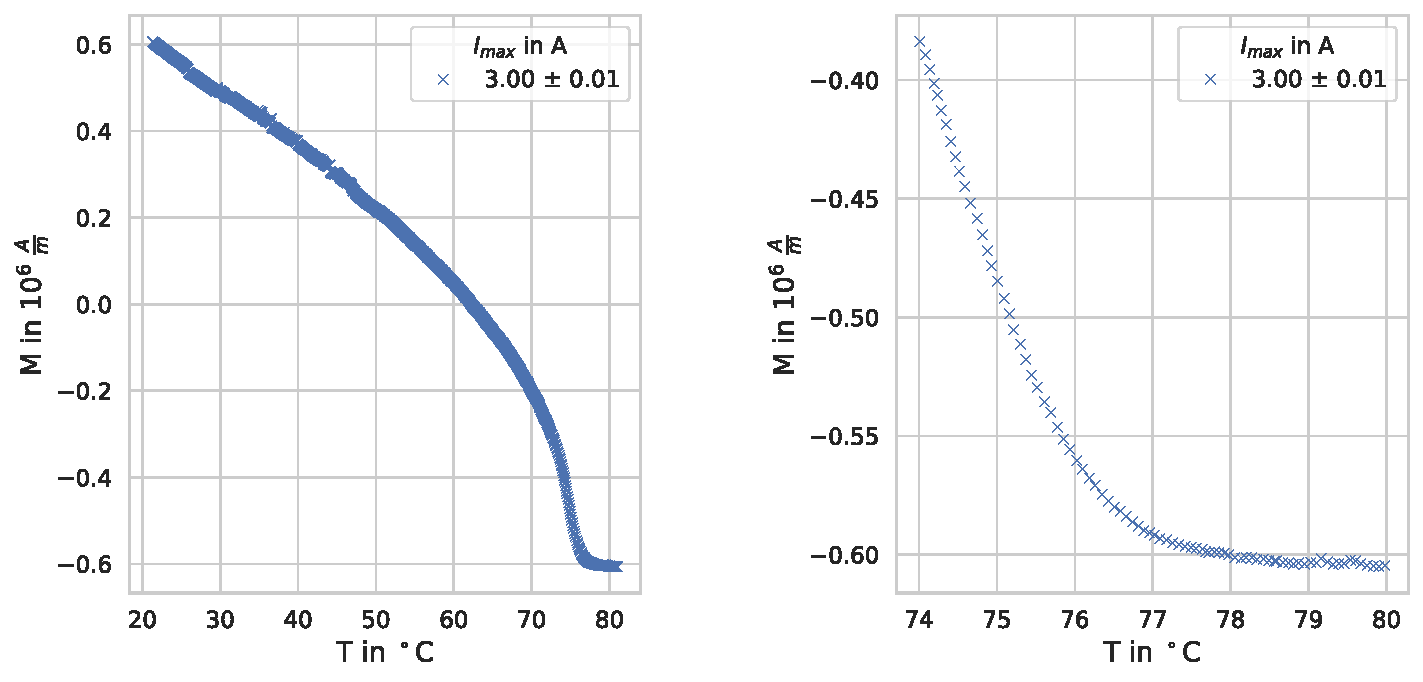
\includegraphics[scale=0.5]{../media/B2.4/3.3.3.pdf}
\caption{Temperaturabhängigkeit der Magnetisierung}
\label{Abb: Temperatur}
\end{figure}

\hypertarget{messungen-am-ringkern-mit-spalt-1}{%
\subsection{Messungen am Ringkern mit Spalt}\label{messungen-am-ringkern-mit-spalt-1}}

\hypertarget{kenngruxf6uxdfen-1}{%
\subsubsection{Kenngrößen}\label{kenngruxf6uxdfen-1}}
Analog zu den Messungen am beheizbaren Ringkern ohne Spalt können die Kenngrößen des Ringkerns mit Spalt ermittelt werden. Diese werden in Tabelle \ref{Tab: kenngr Spalt} dargestellt.

Die Stromstärken \(I_\mathrm{max}\) sind so gewählt, dass die erzeugte Feldstärke in beiden Kernen gleich groß ist. Damit lassen sich die Materialeigenschaften vergleichen.

Dabei fällt auf, dass Remanenz und maximale Magnetisierung bei dem Kern mit Spalt nur etwa halb so groß wie beim Kern ohne Spalt ist. Dafür ist die Koerzitivfeldstärke beim Kern mit Spalt um einen Faktor \(38\) größer. Dies ist auch in der graphischen Darstellung in Abbildung \ref{Abb: Vergleich} ersichtlich.

\begin{table}
\begin{align*}
	I_\mathrm{max} &\text{ in } \mathrm A &
		H_\mathrm{K} &\text{ in }
			{\tiny \left[ \frac{\mathrm A}{\mathrm m} \right] } &
		M_R &\text{ in }
		{\tiny \left[10^6 \frac{\mathrm A}{\mathrm m} \right] } &
		M_\mathrm{max} &\text{ in }
		{\tiny \left[10^6 \frac{\mathrm A}{\mathrm m} \right] }
		\\
	\text{ohne Spalt}\qquad
		3.00 &\pm 0.01 &
		5.71 &\pm 0.46 &
		0.11 &\pm 0.04 &
		0.31 &\pm 0.08
		\\
	\text{mit Spalt}\qquad
		0.94 &\pm 0.01 &
		74.09 &\pm 6.84 &
		0.06 &\pm 0.04 &
		0.12 &\pm 0.07
\end{align*}
\caption{Kenngrößen des Ringkerns mit Spalt}
\label{Tab: kenngr Spalt}
\end{table}

\begin{figure}[ht]
\centering
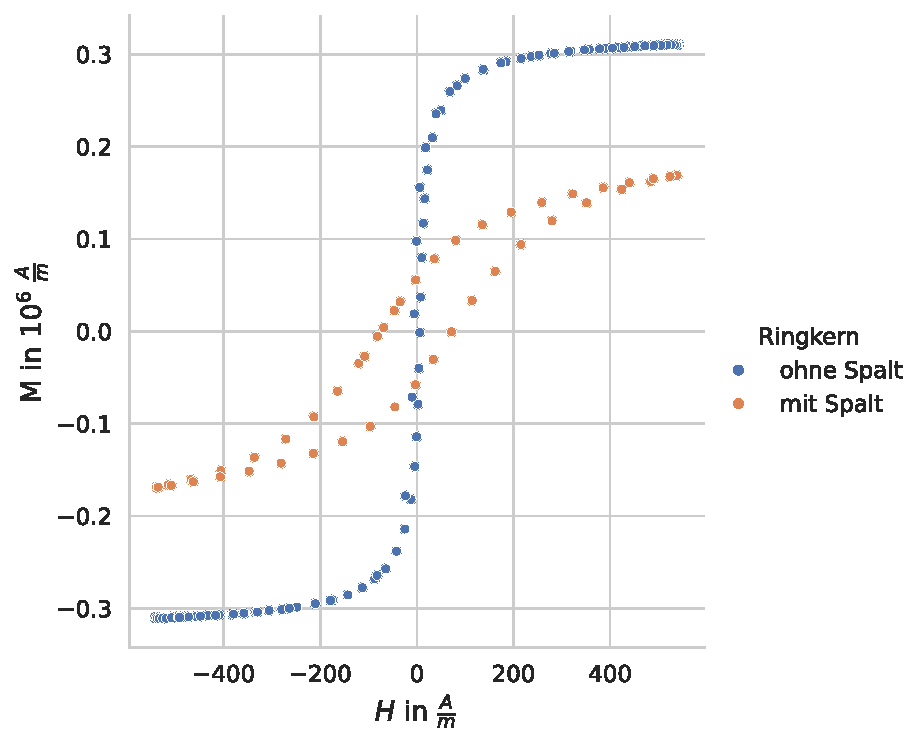
\includegraphics[scale=0.7]{../media/B2.4/3.3.3_comparison.pdf}
\caption{Vergleich der Kerne mit und ohne Spalt}
\label{Abb: Vergleich}
\end{figure}

\hypertarget{entmagnetisierungsfaktor-2}{%
\subsubsection{Entmagnetisierungsfaktor}\label{entmagnetisierungsfaktor-2}}
Aus der Scherung der Hysteresekurven kann nach Gleichung \(\eqref{Hscher}\) die Entmagnetisierungsfeldstärke \(H_\mathrm{ent}\) ermittelt werden.

\begin{figure}[ht]
\centering
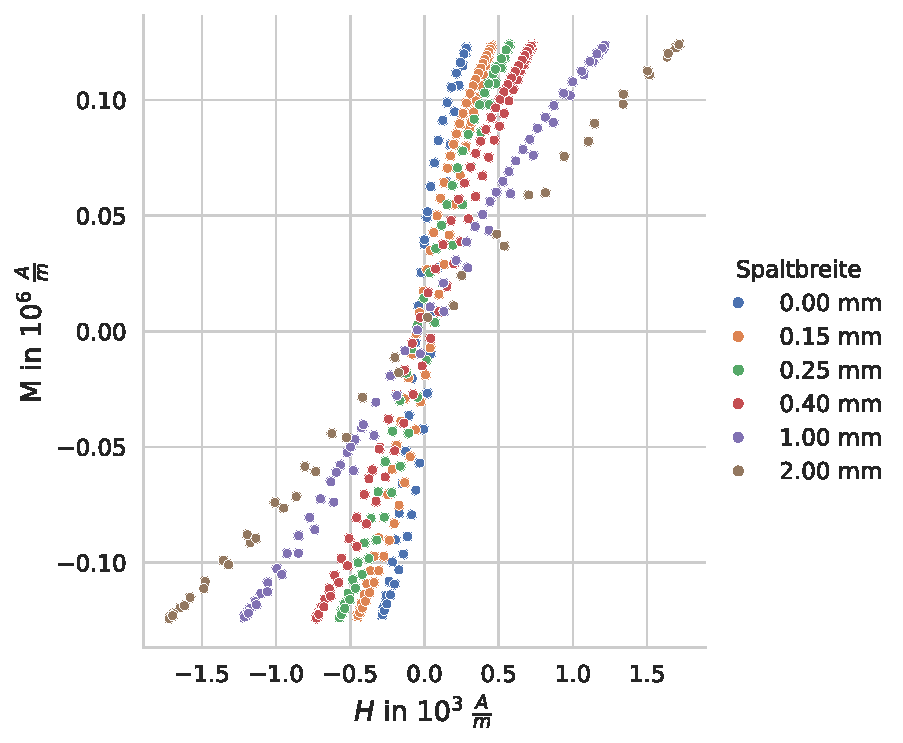
\includegraphics[scale=0.7]{../media/B2.4/3.3.3_overview.pdf}
\caption{gescherte Hysteresekuven}
\label{Abb: Scherung}
\end{figure}

Die maximale Magnetisierung \(M_\mathrm{max} = (0.12\pm 0.08) \cdot 10^6 \mathrm{\frac{A}{m}}\) ist im Rahmen der Messungenauigkeit konstant geblieben. Nach der Definition des Entmagnetisierungsfaktors \eqref{defN} kann damit der experimentelle Entmagnetisierungsfaktor \(N_\mathrm{exp}\) abhängig von der Spaltbreite ermittelt werden. Die Ungenauigkeiten \(\Delta N_\mathrm{exp}\) können durch die Gauß'sche Fehlerfortpflanzung bestimmt werden.

\begin{eqnarray}
    \Delta f &=& \pm\sqrt{
        \sum_{k=1}^j
            \left(
                \frac{\partial f}{\partial x_k} \Delta x_k
            \right)^2
        } \\
    \Delta N_\mathrm{exp} &=&
        \pm\sqrt{
            \left(\frac{\Delta H_\mathrm{ent}}{M_\mathrm{max}}\right)^2
            + \left(\frac{H_\mathrm{ent}\cdot \Delta M_\mathrm{max}}{(M_\mathrm{max})^2}\right)^2       }
\end{eqnarray}

\noindent
Da die Ungenauigkeit der Entmagnetiserungsfeldstärken \(\Delta H_\mathrm{ent}\) sehr viel kleiner als die Ungenauigkeiten der maximalen Magnetisierung \(\Delta M_\mathrm{max}\) sind, wurden erstere in der Berechnung des Entmagnetisierungsfaktors \(N\) vernachlässigt, also \(\Delta H_\mathrm{ent}\approx 0\).

Aus der Spaltbreite \(l_L\) und dem Radius \(R\) des Kerns der theoretische Entmagnetisierungsfaktor \(N_\mathrm{theo}\) nach \(\eqref{N}\) bestimmt werden. Hierbei ist die Gesamtlänge durch den Umfang \(2\pi R\) des Kerns und die Breite des Luftspalts \(l_L\)
bestimmt.

\begin{eqnarray}
    N &=& \frac{l_L}{2\pi R + l_L} 
\end{eqnarray}
Daraus ergeben sich folgende Ergebnisse in Tabelle \ref{Tab: Entmagnetisierung} und Abbildung \ref{Abb: Entmagnetisierung}. Alle Messwerte mit Spalt sind kleiner als die theoretischen Werte, im Rahmen der Messungenauigkeit stimmen sie aber meistens. Dies deutet auf einen systematischen Fehler hin.

Dieser könnte sein, dass das Magnetfeld im Spalt nicht immer homogen ist. Insbesondere bei dem größten Spalt von \(2\mathrm{\,mm}\) ist dies vermutlich der Grund, warum der Messwert so stark abweicht. Dies ist der einzige Wert, der stärker vom theoretischen Wert abweicht, als seine Ungenauigkeit erlaubt.

Weiterhin werden die Abweichungen vom Theoriewert immer größer. Dies deutet darauf hin, dass das Magnetfeld im Spalt ab einer Spaltbreite von \(1\mathrm{\,mm}\) nicht mehr homogen ist.

\begin{figure}[ht]
	\centering
	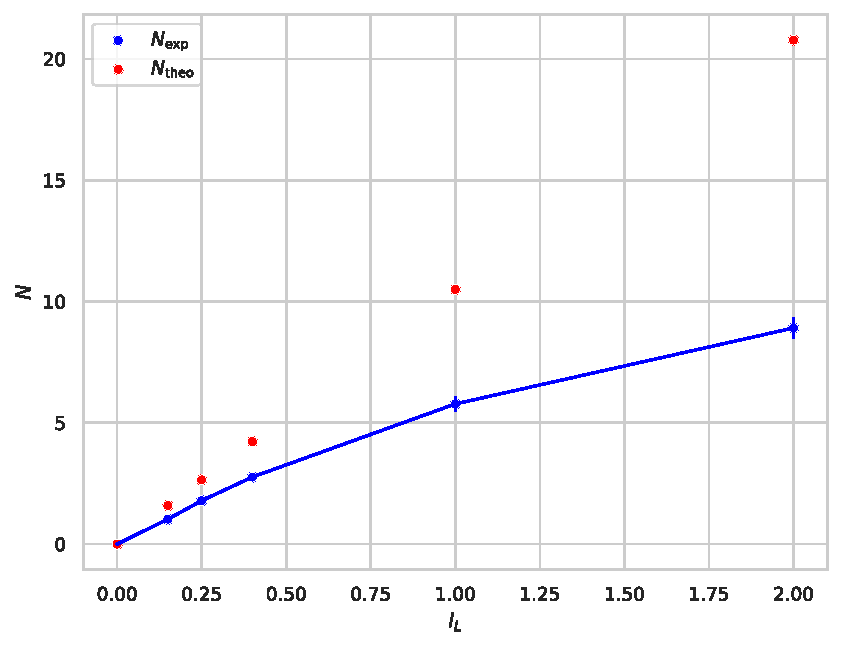
\includegraphics[scale=0.6]{../media/B2.4/3.3.4_N.pdf}
	\caption{Entmagnetisierungsfaktor}
	\label{Abb: Entmagnetisierung}
\end{figure}

\begin{table}
\begin{align*}
	&l_L &
		I_\mathrm{max} &\text{ in } \mathrm A &
		H_\mathrm{ent} &\text{ in }
		{\tiny \left[ 10^3 \frac{\mathrm A}{\mathrm m} \right] } &
		M_\mathrm{max} &\text{ in }
		{\tiny \left[ 10^6 \frac{\mathrm A}{\mathrm m} \right] } &
		N_\mathrm{exp} &\text{ in } [10^{-3}] &
		N_\mathrm{theo} &\text{ in } [10^{-3}]
		\\
	&0.00 \ \mathrm{mm} &
		0.50 &\pm 0.01 &
		0.00 &\pm 0.03 &
		0.12 &\pm 0.08 &
		0.00 &\pm 2.50 &
		0.00\\
	&0.15 \ \mathrm{mm} &
		0.79 &\pm 0.01 &
		0.17 &\pm 0.03 &
		0.12 &\pm 0.08 &
		1.42 &\pm 0.98 &
		1.59\\
	&0.25 \ \mathrm{mm} &
		1.00 &\pm 0.01 &
		0.29 &\pm 0.03 &
		0.12 &\pm 0.07 &
		2.42 &\pm 1.63 &
		2.65\\
	&0.40 \ \mathrm{mm} &
		1.27 &\pm 0.01 &
		0.44 &\pm 0.02 &
		0.12 &\pm 0.07 &
		3.67 &\pm 2.45 &
		4.23\\
	&1.00 \ \mathrm{mm} &
		2.12 &\pm 0.01 &
		0.93 &\pm 0.02 &
		0.12 &\pm 0.07 &
		7.75 &\pm 5.17 &
		10.50\\
	&2.00 \ \mathrm{mm} &
		3.00 &\pm 0.01 &
		1.43 &\pm 0.01 &
		0.12 &\pm 0.06 &
		11.92 &\pm 7.94 &
		20.78
\end{align*}
\caption{Entmagnetisierungsfaktor}
\label{Tab: Entmagnetisierung}
\end{table}

\clearpage
\hypertarget{fazit}{%
\section{Fazit}\label{fazit}}

Insgesamt fällt der Großteil der Ergebnissen wie erwartet aus.

Der Anstieg der Kenngrößen mit steigenden Stromstärke entsprechen den Erwartungen, auch wenn bei der Durchführung es schwierig war die Phase so einzustellen, dass diese nicht stehen bleibt oder rückwärts läuft und man genügend gute Punkte auf der Hysterese erhält. Auffällig bei der Hyteresekurve mit Spalt ist die sehr große Koerzitivfeldstärke im Vergleich zu der Kurve ohne Spalt. Dies weist daraus hin, dass die Kerne aus verschiedenen Materialien bestehen und der Kern mit Spalt vermutlich hartmagnetisch ist, während der beheizbare Ferritkern aus ersten Versuchsteil weichmagnetisch ist.

Die Kurven der differentiellen Suszeptibilität ähneln sich insofern, dass beide bis zu einem Maximum ansteigen und dann, bei betragsmäßig höheren \(H\), wieder abfallen. Allerdings haben wir eine ca \(20\)-fache Abweichung zwischen beide Messungen und der Plot oszilliert leicht. Diese Ungleichmäßigkeiten lassen sich bei manuellem Regeln der Stromstärke nicht vermeiden. Dennoch kann man den Verlauf der Kurven als physikalisch sinnvoll beurteilen. Was aber dazu geführt hat, dass die zweite Messung negative Magnetisierungswerte angenommen hat, ist nicht geklärt, denn eigentlich war die Phase an dem oberen Sättigungspunkt fixiert. Hier gab es offensichtlich einen systematischen Fehler.

Die zeitaufwändige Temperaturmessung liefert einer der besten Ergebnissen, nämlich eine um \(T_{c}\) verschobene und gespiegelte Wurzelfunktion so wie die Landau-Theorie es vorhergesagt hat. Die Curie-Temperatur hier beträgt \((76.5 \pm 0.5) \ ^\circ\mathrm C\).

Schließlich trifft die Messung des Entmagnetisierungsfaktors die erwarteten theoretischen Werte ziemlich gut. Es lässt sich vermuten, dass das Magnetfeld in einem Spalt von \(1\mathrm{\,mm}\) nicht mehr homogen ist.

\clearpage
\hypertarget{literaturverzeichnis}{%
\section{Literaturverzeichnis}\label{literaturverzeichnis}}
\begin{thebibliography}{9}
	\bibitem{Jackson}
J. D. Jackson, Classical Elektrodynamics, New York: John Wiley \& Sons, 1962
	\bibitem{Kittel}
		C. Kittel, Einführung in die Festkörperphysik, München: Oldenbourg Verlag, 2005
	\bibitem{Kneller}
		E. Kneller, Ferromagnetismus, Berlin Heidelberg: Springer Verlag, 1962
	\bibitem{Reith}
		W. Reith, Bergmann-Schaefer. Lehrbuch der Experimentalphysik: Elektromagnetismus, Bd. 2, Berlin: Walter de Gruyter Verlag, 2006
	\bibitem{Hunklinger}
		S. Hunklinger, Festkörperphysik, München: Oldenbourg Verlag, 2011
	\bibitem{Gross}
		R. Gross und A. Marx, Festkörperphysik, München: Oldenbourg Verlag, 2012
	\bibitem{Fink}
		M. Fink, R.-D. Heuer und H. Kleinpoppen, Bergmann-Schaefer. Bestandteile der Materie, Bd. 4, W. Raith, Hrsg., Berlin: Walter de Gruyter Verlag, 2003
	\bibitem{Uni}
		Universität zu Köln, ``Anleitung zum Versuch 2.4 -- Magnetisierung eines Ferrits'', Juni 2013, Online verfügbar unter \url{http://www.ph2.uni-koeln.de/fileadmin/Lehre/PraktikumB/B2.4.pdf}
\end{thebibliography}

\end{document}
